\chapter{Anàlisi electromagnètic}

El programa 4NEC, basat en popular sistema de modelat anomenat \textit{NEC} que resol l'equació integral del camp elèctric(EFIE) i l'equació integral del camp magnètic(MFIE) permet fer un anàlisis força acurat d'antenes de fil. Així doncs, s'empra aquest programa \textit{open-source} per dur a terme un anàlisi per a  les diverses configuracions d'antenes comentades.

\section{Antena dipol en $\lambda/2$}

En aquesta secció s'estudia i analitza una antena dipol en $\lambda/2$ per a diverses situacions.

 \subsection{En espai lliure}

 Per l'antena dipol comentada situada en un espai lliure s'analitzen els digrames de radiació així com la directivitat i la impedància d'entrada.

 	\textbf{Diagrames de Radiació}

	\begin{figure}[H]
	\centering
	  \begin{subfigure}[b]{0.32\textwidth}
	  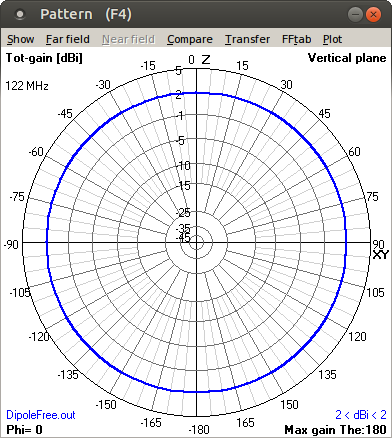
\includegraphics[width=\textwidth]{./images/1.Dypole_Free/1_vertical.png}
	  \caption{}
	  \label{1diag1}
	  \end{subfigure}
	  \qquad %~ %add desired spacing between  images, e. g. ~, \quad,  \qquad, \hfill etc. 
	  \begin{subfigure}[b]{0.32\textwidth}
	  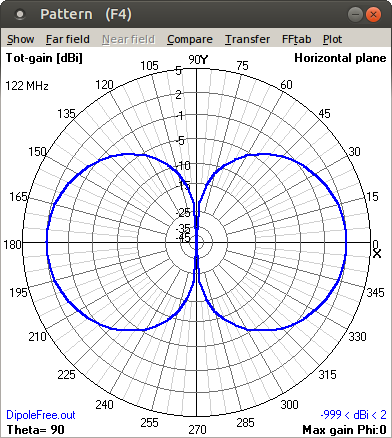
\includegraphics[width=\textwidth]{./images/1.Dypole_Free/1_horizontal.png}
	  \caption{}
	  \label{1diag2}
	  \end{subfigure}
	  \vspace{10pt}
	\caption{Diagrames de Radiació d'antena dipol en $\lambda/2$ en espai lliure}
	\label{diag1}
	\end{figure}

	\begin{figure}[H]
	\centering
	  \begin{subfigure}[b]{0.53\textwidth}
	  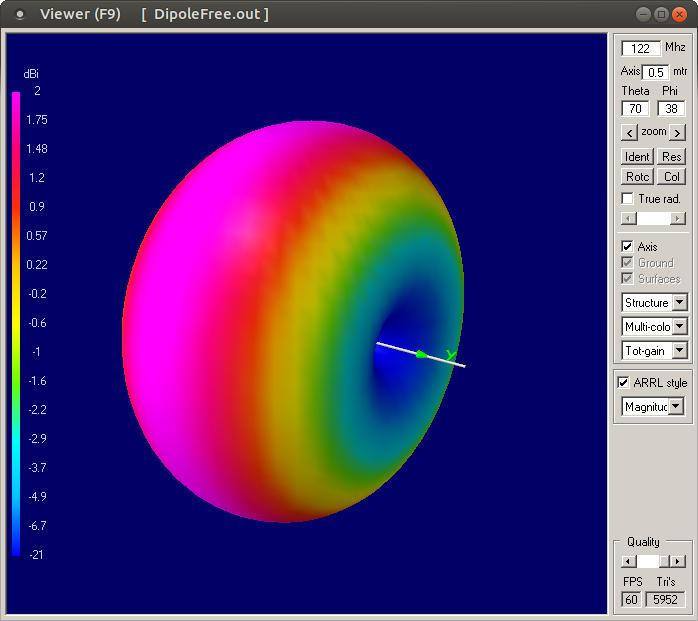
\includegraphics[width=\textwidth]{./images/1.Dypole_Free/1_3d.png}
	  \caption{Digrama de Radiació 3D d'antena dipol en $\lambda/2$ en espai lliure}
	  \label{1diag3d}
	  \end{subfigure}
	  \qquad %~ %add desired spacing between  images, e. g. ~, \quad,  \qquad, \hfill etc. 
	  \begin{subfigure}[b]{0.32\textwidth}
	  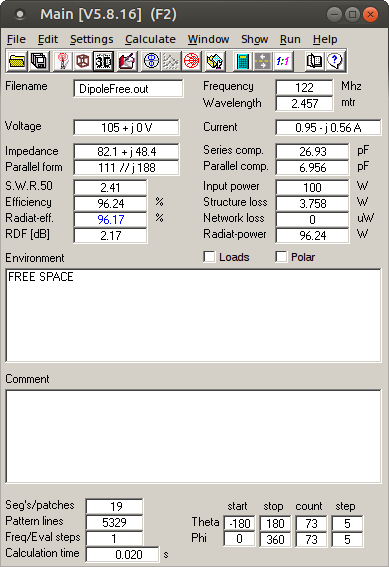
\includegraphics[width=\textwidth]{./images/1.Dypole_Free/1_menu.png}
	  \caption{Dades de l'antena dipol en $\lambda/2$ en espai lliure}
	  \label{1menu}
	  \end{subfigure}
	  \vspace{10pt}
	\caption{}
	\label{diag2}
	\end{figure}

	\textbf{Directivitat de l'antena:} $ D=2.17 dB$. \\
	\textbf{Impedància d'entrada:} $ Z_0=82.1+j48.4 \si{\ohm}$.


 \subsection{A certa distància d’un pla conductor perfecte}

  Per l'antena dipol comentada situada a una certa distància d'un pla conductor s'analitzen els diagrames de radiació així com la directivitat i la impedància d'entrada. 

 \textbf{Diagrames de Radiació}

 	\begin{figure}[H]
	\centering
	  \begin{subfigure}[b]{0.32\textwidth}
	  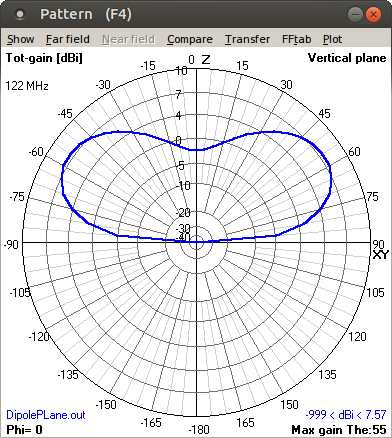
\includegraphics[width=\textwidth]{./images/2.Dypole_overPlane/2_vertical.png}
	  \caption{}
	  \label{2diag1}
	  \end{subfigure}
	  \qquad %~ %add desired spacing between  images, e. g. ~, \quad,  \qquad, \hfill etc. 
	  \begin{subfigure}[b]{0.32\textwidth}
	  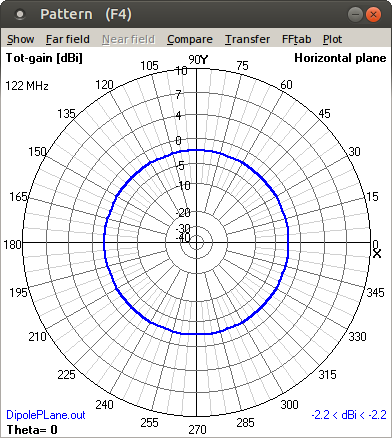
\includegraphics[width=\textwidth]{./images/2.Dypole_overPlane/2_horizontal.png}
	  \caption{}
	  \label{2diag2}
	  \end{subfigure}
	  \vspace{10pt}
	\caption{Diagrames de Radiació d'antena dipol en $\lambda/2$ a una certa distància d'un pla conductor}
	\label{diag3}
	\end{figure}

	\begin{figure}[H]
	\centering
	  \begin{subfigure}[b]{0.53\textwidth}
	  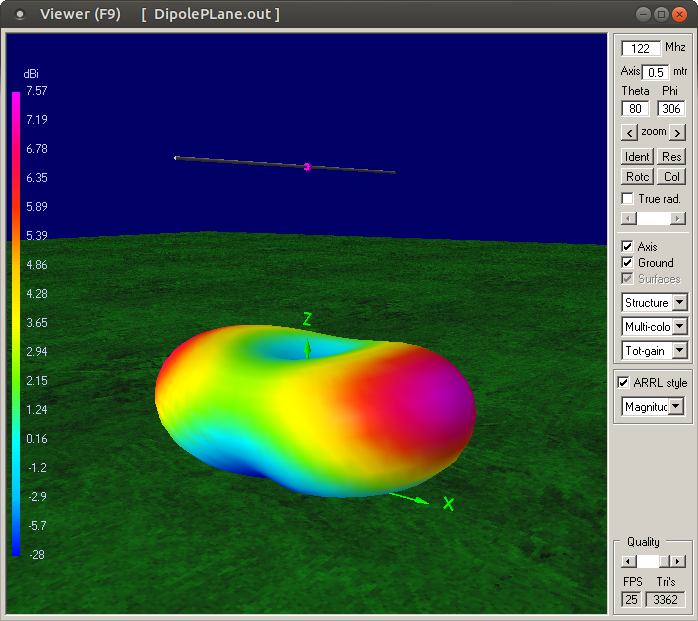
\includegraphics[width=\textwidth]{./images/2.Dypole_overPlane/2_3d.png}
	  \caption{Digrama de Radiació 3D d'antena dipol en $\lambda/2$ a una certa distància d'un pla conductor}
	  \label{2diag3d}
	  \end{subfigure}
	  \qquad %~ %add desired s2acing between  images, e. g. ~, \quad,  \qquad, \hfill etc. 
	  \begin{subfigure}[b]{0.33\textwidth}
	  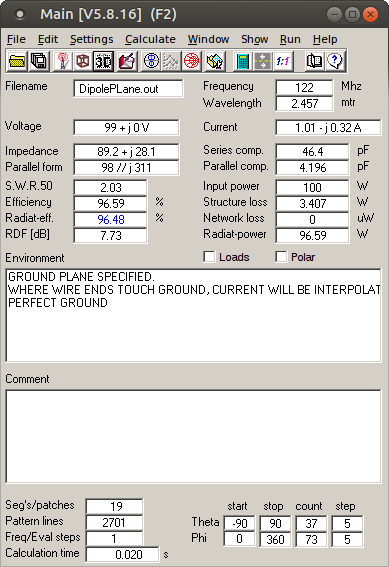
\includegraphics[width=\textwidth]{./images/2.Dypole_overPlane/menu.png}
	  \caption{Dades de l'antena dipol en $\lambda/2$ a distància d'un pla conductor}
	  \label{2menu}
	  \end{subfigure}
	  \vspace{10pt}
	\caption{}
	\label{diag4}
	\end{figure}

	\textbf{Directivitat de l'antena:} $ D=7.73 dB$. \\
	\textbf{Impedància d'entrada:} $ Z_0=89.2+j28.1 \si{\ohm}$.


 \subsection{Sobre un cilindre metàl·lic}

  Per l'antena dipol comentada situada sobre un cilindre metàl·lic s'analitzen els diagrames de radiació així com la directivitat i la impedància d'entrada.

  \textbf{Diagrames de Radiació}

	\begin{figure}[H]
	\centering
	  \begin{subfigure}[b]{0.32\textwidth}
	  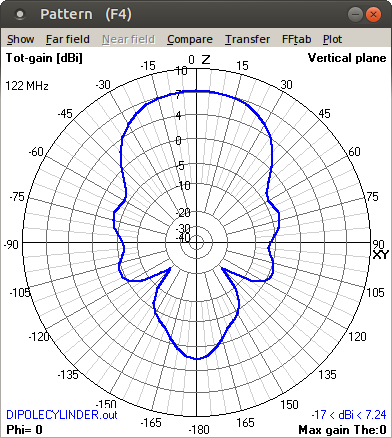
\includegraphics[width=\textwidth]{./images/3.Dypole_cylinder/3_vertical.png}
	  \caption{}
	  \label{1diag1}
	  \end{subfigure}
	  \qquad %~ %add desired spacing between  images, e. g. ~, \quad,  \qquad, \hfill etc. 
	  \begin{subfigure}[b]{0.32\textwidth}
	  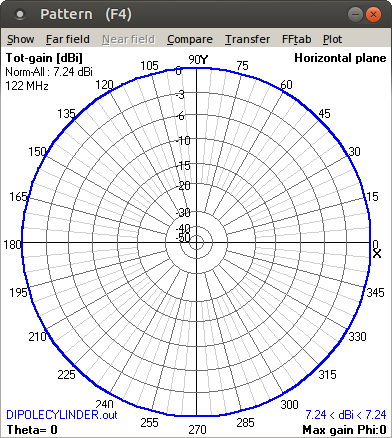
\includegraphics[width=\textwidth]{./images/3.Dypole_cylinder/3_horizontal.png}
	  \caption{}
	  \label{1diag2}
	  \end{subfigure}
	  \vspace{10pt}
	\caption{Diagrames de Radiació d'antena dipol en $\lambda/2$ sobre un cilindre metàl·lic}
	\label{diag1}
	\end{figure}

	\begin{figure}[H]
	\centering
	  \begin{subfigure}[b]{0.53\textwidth}
	  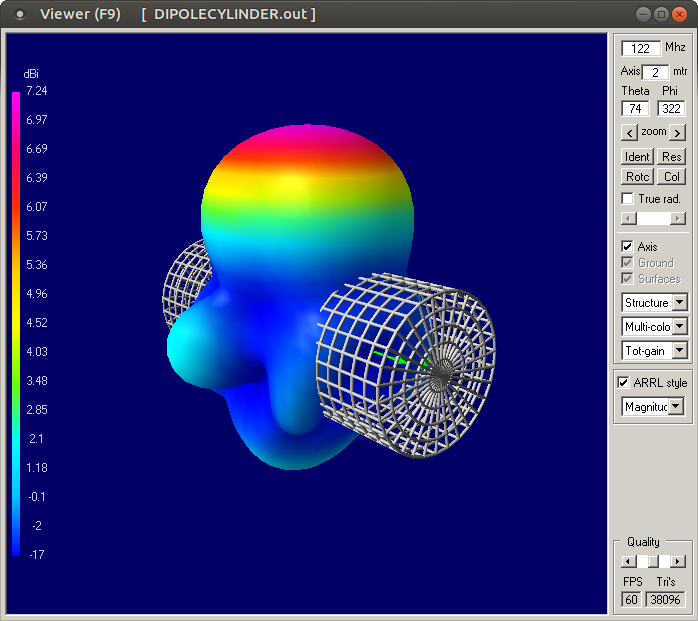
\includegraphics[width=\textwidth]{./images/3.Dypole_cylinder/3_3d.png}
	  \caption{Digrama de Radiació 3D d'antena dipol en $\lambda/2$ sobre un cilindre metàl·lic}
	  \label{1diag3d}
	  \end{subfigure}
	  \qquad %~ %add desired spacing between  images, e. g. ~, \quad,  \qquad, \hfill etc. 
	  \begin{subfigure}[b]{0.32\textwidth}
	  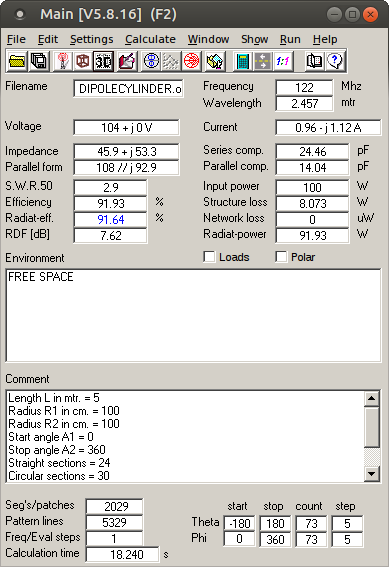
\includegraphics[width=\textwidth]{./images/3.Dypole_cylinder/3_menu.png}
	  \caption{Dades de l'antena dipol en $\lambda/2$ sobre un cilindre metàl·lic}
	  \label{1menu}
	  \end{subfigure}
	  \vspace{10pt}
	\caption{}
	\label{diag2}
	\end{figure}

	\textbf{Directivitat de l'antena:} $ D=7.62 dB$. \\
	\textbf{Impedància d'entrada:} $ Z_0=45.9+j53.3 \si{\ohm}$.


 \section{Antena monopol en $\lambda/4$}

 En aquesta secció s'estudia i analitza una antena monopol en $\lambda/4$ per a diverses situacions. 

\newpage
\subsection{Sobre un pla conductor perfecte}

  Per l'antena monopol comentada situada sobre un pla conductor s'analitzen els diagrames de radiació així com la directivitat i la impedància d'entrada.

 \textbf{Diagrames de Radiació}

 	\begin{figure}[H]
	\centering
	  \begin{subfigure}[b]{0.32\textwidth}
	  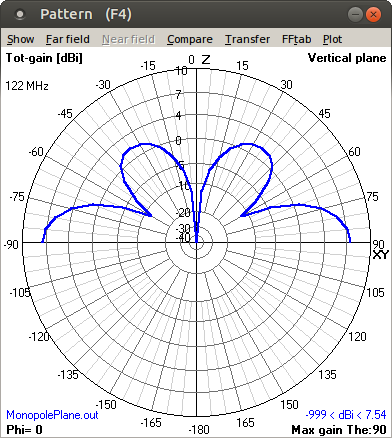
\includegraphics[width=\textwidth]{./images/4.Monopole_plane/vertical.png}
	  \caption{}
	  \label{2diag1}
	  \end{subfigure}
	  \qquad %~ %add desired spacing between  images, e. g. ~, \quad,  \qquad, \hfill etc. 
	  \begin{subfigure}[b]{0.32\textwidth}
	  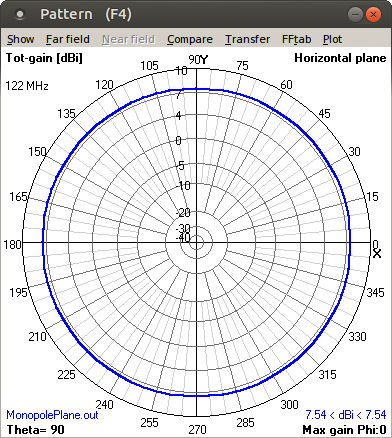
\includegraphics[width=\textwidth]{./images/4.Monopole_plane/horizontal.png}
	  \caption{}
	  \label{2diag2}
	  \end{subfigure}
	  \vspace{10pt}
	\caption{Diagrames de Radiació d'antena monopol en $\lambda/4$ sobre un pla conductor}
	\label{diag3}
	\end{figure}

	\begin{figure}[H]
	\centering
	  \begin{subfigure}[b]{0.53\textwidth}
	  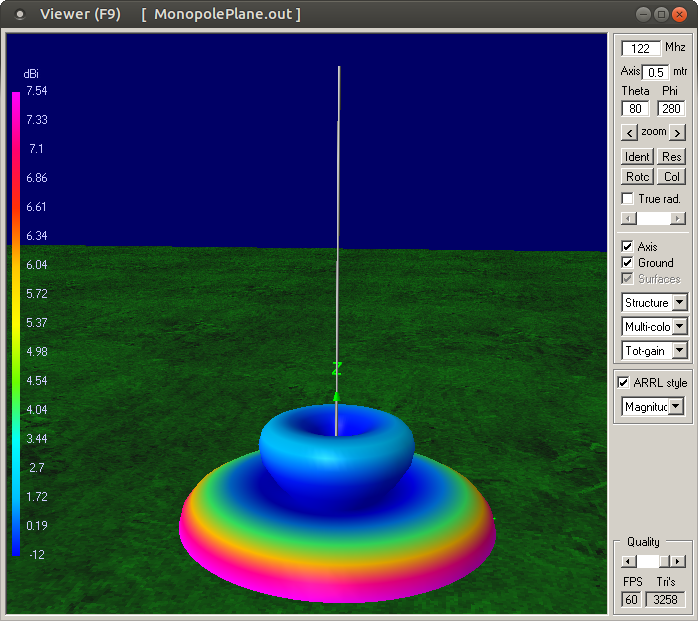
\includegraphics[width=\textwidth]{./images/4.Monopole_plane/3d.png}
	  \caption{Digrama de Radiació 3D d'antena monopol en $\lambda/4$ sobre un pla conductor}
	  \label{2diag3d}
	  \end{subfigure}
	  \qquad %~ %add desired spacing between  images, e. g. ~, \quad,  \qquad, \hfill etc. 
	  \begin{subfigure}[b]{0.32\textwidth}
	  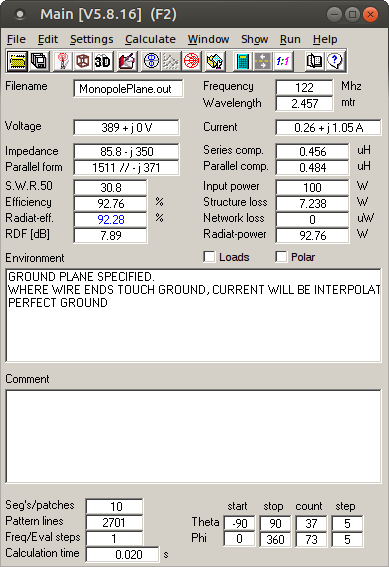
\includegraphics[width=\textwidth]{./images/4.Monopole_plane/menu.png}
	  \caption{Dades de l'antena monopol en $\lambda/4$ sobre un pla conductor}
	  \label{2menu}
	  \end{subfigure}
	  \vspace{10pt}
	\caption{}
	\label{diag4}
	\end{figure}

	\textbf{Directivitat de l'antena:} $ D=7.89 dB$. \\
	\textbf{Impedància d'entrada:} $ Z_0=85.8-j350 \si{\ohm}$.

\newpage
 \subsection{Sobre un cilindre metàl·lic}

  Per l'antena monopol comentada situada sobre un cilindre metàl·lic s'analitzen els diagrames de radiació així com la directivitat i la impedància d'entrada.

  \textbf{Diagrames de Radiació}

	\begin{figure}[H]
	\centering
	  \begin{subfigure}[b]{0.32\textwidth}
	  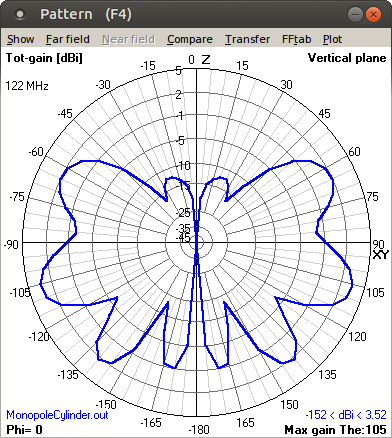
\includegraphics[width=\textwidth]{./images/5.Monopole_cylinder/vertical.png}
	  \caption{}
	  \label{1diag1}
	  \end{subfigure}
	  \qquad %~ %add desired spacing between  images, e. g. ~, \quad,  \qquad, \hfill etc. 
	  \begin{subfigure}[b]{0.32\textwidth}
	  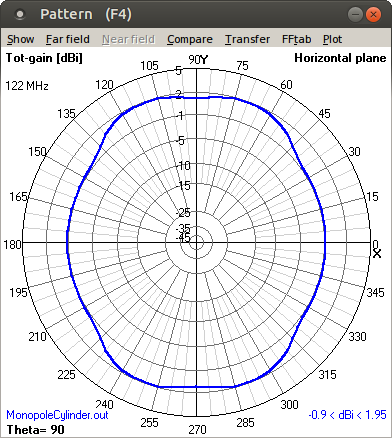
\includegraphics[width=\textwidth]{./images/5.Monopole_cylinder/horizontal.png}
	  \caption{}
	  \label{1diag2}
	  \end{subfigure}
	  \vspace{10pt}
	\caption{Diagrames de Radiació d'antena monopol en $\lambda/4$ sobre un cilindre metàl·lic}
	\label{diag1}
	\end{figure}

	\begin{figure}[H]
	\centering
	  \begin{subfigure}[b]{0.53\textwidth}
	  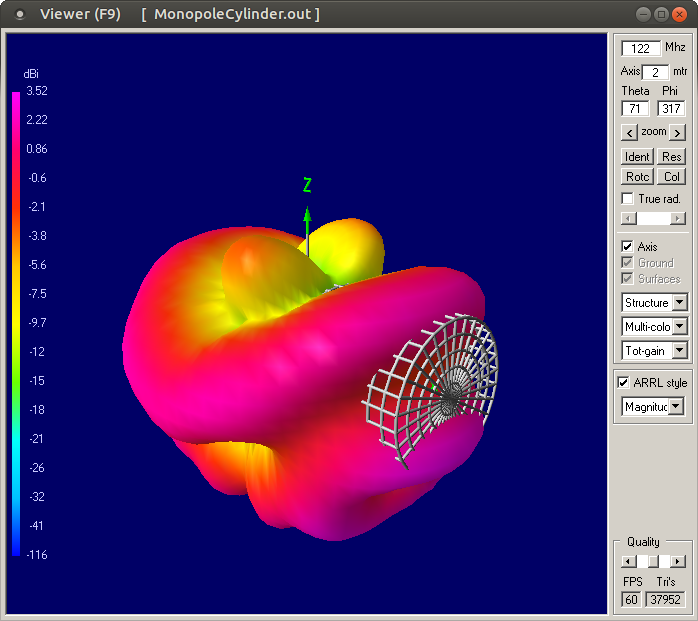
\includegraphics[width=\textwidth]{./images/5.Monopole_cylinder/3d.png}
	  \caption{Digrama de Radiació 3D d'antena monopol en $\lambda/4$ sobre un cilindre metàl·lic}
	  \label{1diag3d}
	  \end{subfigure}
	  \qquad %~ %add desired spacing between  images, e. g. ~, \quad,  \qquad, \hfill etc. 
	  \begin{subfigure}[b]{0.32\textwidth}
	  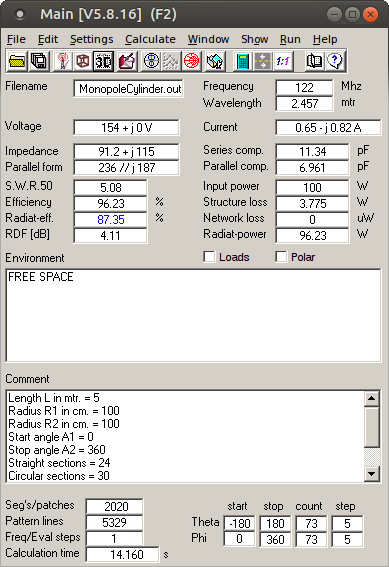
\includegraphics[width=\textwidth]{./images/5.Monopole_cylinder/menu.png}
	  \caption{Dades de l'antena monopol en $\lambda/4$ sobre un cilindre metàl·lic}
	  \label{1menu}
	  \end{subfigure}
	  \vspace{10pt}
	\caption{}
	\label{diag2}
	\end{figure}

	\textbf{Directivitat de l'antena:} $ D=4.11 dB$. \\
	\textbf{Impedància d'entrada:} $ Z_0=91.2+j115 \si{\ohm}$.
